\chapter{Proposed Methodology}
Our project will be divided into two distinct phases. Phase 1 will involve the development of a Nepali Language model dedicated to text generation and spelling correction. Once Phase 1 is successfully completed, we will proceed to Phase 2, which will focus on the development of Nepali Automatic Speech Recognition.

\section{Nepali Language Model for Text Generation}
During this phase, our focus will be on creating a Nepali language model for text generation. To achieve this, we will work on building both a transformer model and a GPT-based model. The architectures of these models are outlined below:

\subsection{Transformer based model for text generation}
In this phase, our transformer-based model will utilize a standard transformer module based on the paper "Attention is All You Need" \cite{NIPS2017_3f5ee243} as discussed in the literature review section. However, for the language generation task, we will specifically train only the transformer encoder. The objective of language modeling is to estimate the probability of a given word following a sequence of words.

The model architecture involves passing a sequence of tokens through an embedding layer, which is then followed by a positional encoding layer to capture the word order. The next steps include employing multi-head attention and a feed-forward network, as depicted in the figure below. To ensure effective modeling, we will utilize six layers of the transformer encoder.

\begin{figure}[H]
    \centering
    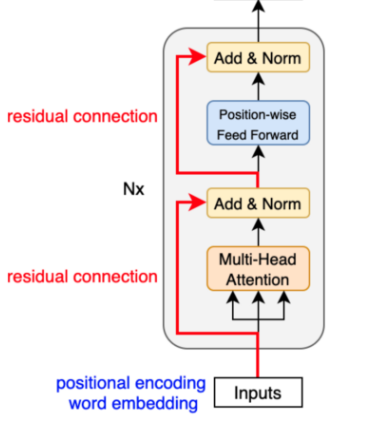
\includegraphics[scale = 0.7]{proposed_methodology/transformer_encoder.png}
    \caption{Transformer Encoder (src: https://kikaben.com/transformers-encoder-decoder/)}
    \label{fig:Transformer Encoder (src: https://kikaben.com/transformers-encoder-decoder/)}
\end{figure}

\section{Spelling Correction}

\section{Nepali Automatic Speech Recognition}
The audio input feature in the Transformer architecture for speech recognition is a sequence of Mel-frequency cepstral coefficients (MFCCs) that are extracted from the audio signal. MFCCs are commonly used in speech recognition systems as they capture the spectral envelope of the speech signal and are robust to noise and channel distortions. Other description of the architecture is same as in the "Attention is All You Need" \cite{NIPS2017_3f5ee243}.

\begin{figure}[H]
    \centering
    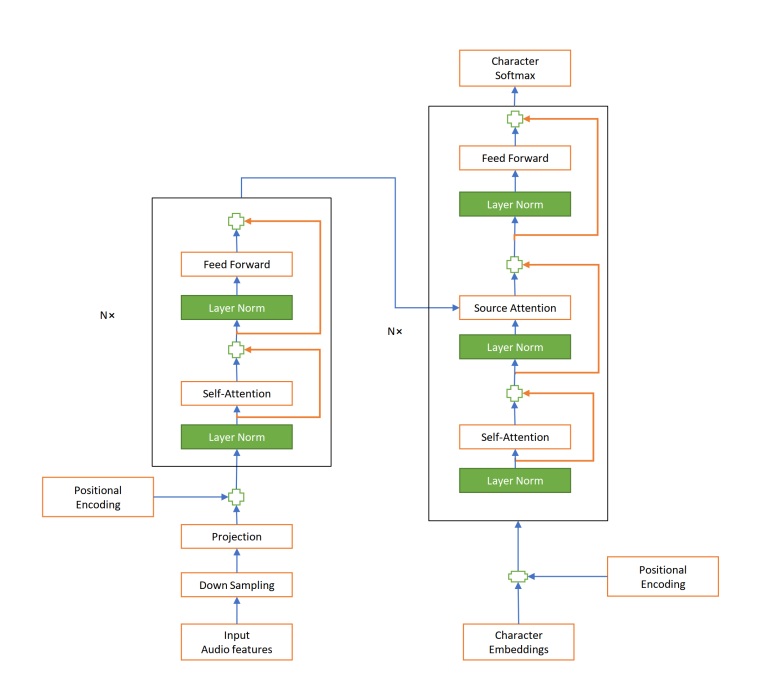
\includegraphics[scale = 0.6]{proposed_methodology/asr_transformer.png}
    \caption{Transformer Network for ASR \cite{pham2019very}}
    \label{fig:Transformer Network for ASR}
\end{figure}



